%% LaTeX Beamer presentation template (requires beamer package)
%% see http://latex-beamer.sourceforge.net/
%% idea contributed by H. Turgut Uyar
%% template based on a template by Till Tantau
%% this template is still evolving - it might differ in future releases!

\documentclass[compress]{beamer}

\mode<presentation>
{
  \usetheme{Singapore}

% \setbeamercovered{transparent}
  \setbeamertemplate{footline}[frame number]
}

\usepackage{ctex}

\usepackage{amsmath}
\usepackage{amssymb}

\usepackage{longtable}
\usepackage{xcolor}
\usepackage[english]{babel}
\usepackage{hyperref}

\newcommand{\tabincell}[2]{\begin{tabular}{@{}#1@{}}#2\end{tabular}}

%\usepackage{mathptmx}
\definecolor{orange}{rgb}{1,0.5,0}

  \defbeamertemplate*{frametitle}{smoothbars theme}
  {%
    \nointerlineskip%
    \begin{beamercolorbox}[wd=\paperwidth,leftskip=.3cm,rightskip=.3cm plus1fil,vmode]{frametitle}
      \vskip.3ex
      \usebeamerfont*{frametitle}\insertframetitle%
      \vskip.3ex
    \end{beamercolorbox}%
  }

% font definitions, try \usepackage{ae} instead of the following
% three lines if you don't like this look
% \usepackage{mathptmx}
% \usepackage[scaled=.90]{helvet}
% \usepackage{courier}

% \usefonttheme[onlymath]{serif}
% \usefonttheme{professionalfonts}

% \usepackage[T1]{fontenc}


\title{{Tutorial for Graph Algorithm}}
% \subtitle{{--- }}

% - Use the \inst{?} command only if the authors have different affiliation.
% \author{F.~Author\inst{1} \and S.~Another\inst{2}}
\author{Hengfeng Wei}

% - Use the \inst command only if there are several affiliations.
% - Keep it simple, no one is interested in your street address.
\institute[Universities of]
{
  hengxin0912@gmail.com
}

\date{December 19, 2011}

% This is only inserted into the PDF information catalog. Can be left out.
%\subject{Talks}

% If you have a file called "university-logo-filename.xxx", where xxx
% is a graphic format that can be processed by latex or pdflatex,
% resp., then you can add a logo as follows:

%\pgfdeclareimage[height=1.2cm]{university-logo}{figure/nju}
%\logo{\pgfuseimage{university-logo}}

% Delete this, if you do not want the table of contents to pop up at
% the beginning of each subsection:
\AtBeginSubsection[]
{
  \begin{frame}<beamer>
    \frametitle{Outline}
    \tableofcontents[currentsection,currentsubsection]
  \end{frame}
}

% If you wish to uncover everything in a step-wise fashion, uncomment
% the following command:

%\beamerdefaultoverlayspecification{<+->}
\begin{document}

\begin{frame}
  \titlepage
\end{frame}

\begin{frame}
  \frametitle{Outline}
  \tableofcontents
% You might wish to add the option [pausesections]
\end{frame}


%%%%%%%%%%%%%%%%%%%%%%%%%%%%%%%%%%%%%%%%%%%%%%%%%%%%%%%%%%%%%%%%%%%%%
%%%%%%%%%%%%%%%%%%%%%% BFS and DFS %%%%%%%%%%%%%%%%%%%%%%%%%%%%%%%%%%%%
\section{BFS and DFS}

\begin{frame}
  \frametitle{BFS and DFS}

  \begin{quote}
    \textcolor{blue}{``For fundamental achievements in the design and analysis of algorithms and data structures.''}

    \hfill {--- Turing Award 1986}
  \end{quote}

  \begin{columns}
    \begin{column}{0.50\textwidth}
      \begin{figure}
        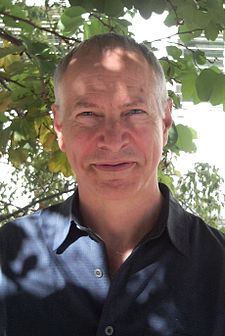
\includegraphics[scale=0.30]{figure/bfs_dfs/Tarjan}
        \caption{{\scriptsize Robert Endre Tarjan (April 30, 1948).}}
        \label{fig:Tarjan}
      \end{figure}
    \end{column}

    \begin{column}{0.50\textwidth}
      \begin{figure}
        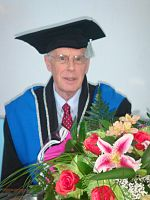
\includegraphics[scale=0.50]{figure/bfs_dfs/hopcroft}
        \caption{{\scriptsize John Edward Hopcroft (October 7, 1939)}.}
        \label{fig:hopcroft}
      \end{figure}
    \end{column}
  \end{columns}

\end{frame}


     %%%%%%%% Exploring types of edges on both BFS and DFS %%%%%%%
\subsection{Exploring Types of Edges on Both BFS and DFS}

\begin{frame}
  \frametitle{Types of edges on DFS}

  \begin{columns}
    \begin{column}{0.50\textwidth}
      \textcolor{purple}{DFS on digraph:}
      \begin{figure}
        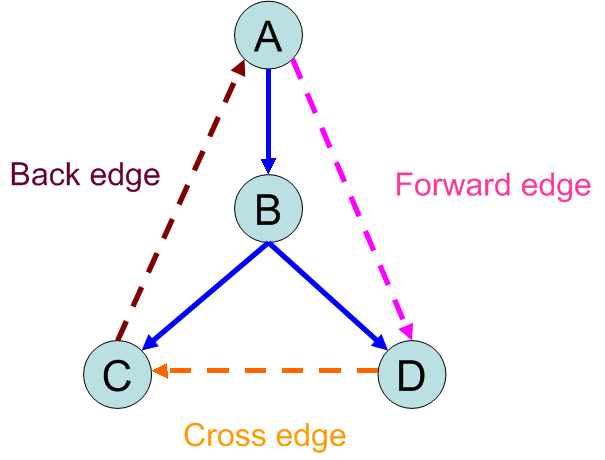
\includegraphics[scale=0.30]{figure/bfs_dfs/dfsdi}
        \caption{{\scriptsize DFS on digraph.}}
        \label{fig:dfsdi}
      \end{figure}
    \end{column}

    \begin{column}{0.50\textwidth}
      \textcolor{purple}{DFS on undirected graph  \\ ([\textcolor{blue}{$P_{380}$ 7.28}]):}
      \begin{figure}
        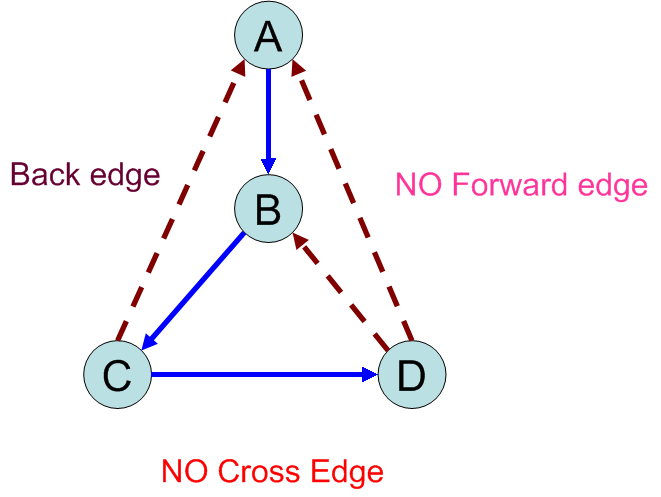
\includegraphics[scale=0.30]{figure/bfs_dfs/dfsundirected}
        \caption{{\scriptsize DFS on undirected graph.}}
        \label{fig:dfsundirected}
      \end{figure}
    \end{column}
  \end{columns}
      
\end{frame}


\begin{frame}
  \frametitle{Types of edges on BFS}

  \begin{columns}
    \begin{column}{0.50\textwidth}
      \textcolor{purple}{BFS on digraph:}
      \begin{figure}
        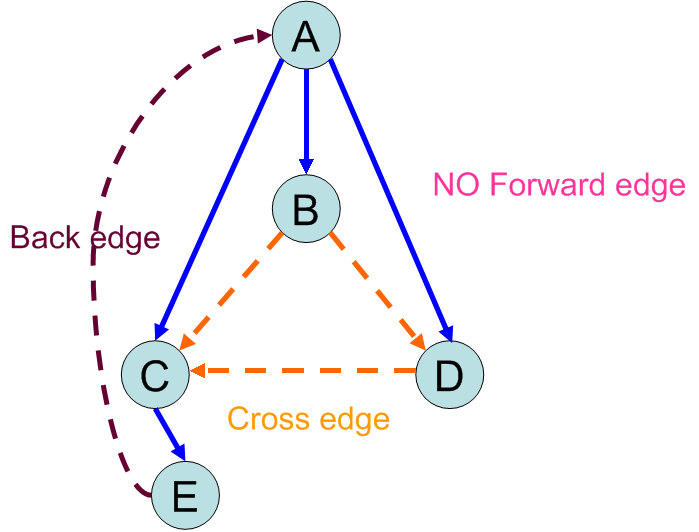
\includegraphics[scale=0.30]{figure/bfs_dfs/bfsdi}
        \caption{{\scriptsize BFS on digraph.}}
        \label{fig:bfsdi}
      \end{figure}
    \end{column}
  
    \begin{column}{0.50\textwidth}
      \textcolor{purple}{BFS on undirected graph:}
      \begin{figure}
        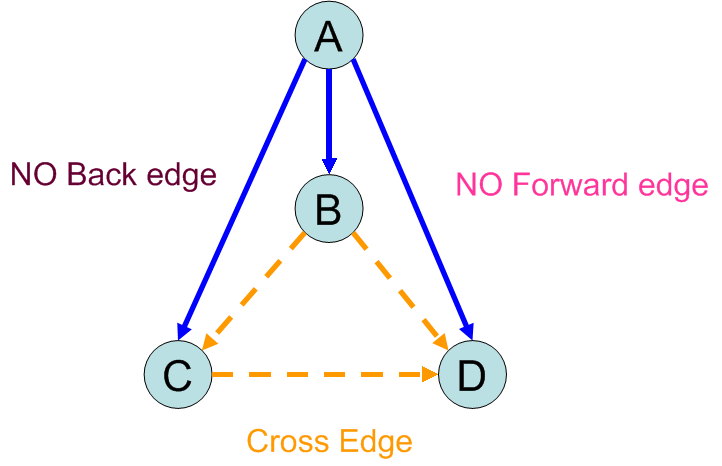
\includegraphics[scale=0.30]{figure/bfs_dfs/bfsundirected}
        \caption{{\scriptsize BFS on undirected graph.}}
        \label{fig:bfsundirected}
      \end{figure}
    \end{column}
  \end{columns}
  
\end{frame}



\begin{frame}
  \frametitle{Cycle detection problems}

  \begin{table}
    \begin{tabular}{|c|c|c|}
      \hline
                & Undirected graph          & Directed graph ([\textcolor{blue}{$P_{379}$ 7.17}])           \\ \hline
      BFS       & \tabincell{c}{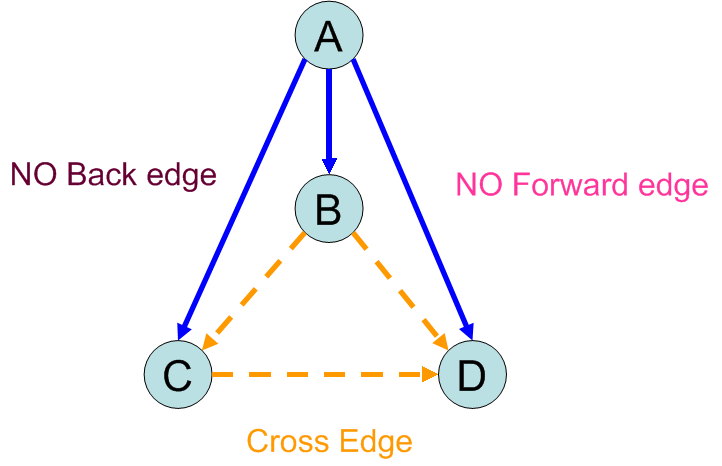
\includegraphics[scale=0.20]{figure/bfs_dfs/bfsundirected} \\ (\textcolor{red}{Cross edge})}
                & \tabincell{c}{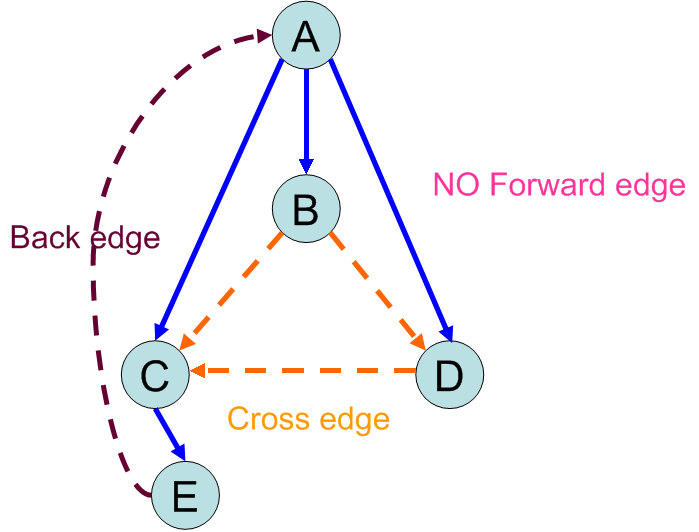
\includegraphics[scale=0.20]{figure/bfs_dfs/bfsdi} \\ (\textcolor{blue}{Back edge?})}            \\ \hline
      DFS       & \tabincell{c}{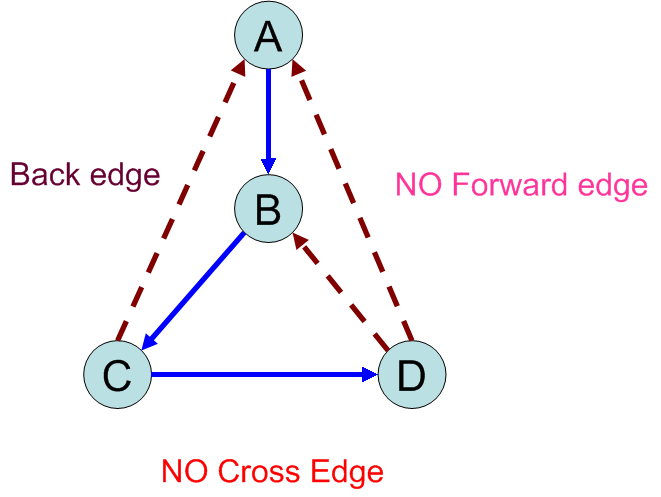
\includegraphics[scale=0.20]{figure/bfs_dfs/dfsundirected} \\ \textcolor{red}{Back edge}}
                & \tabincell{c}{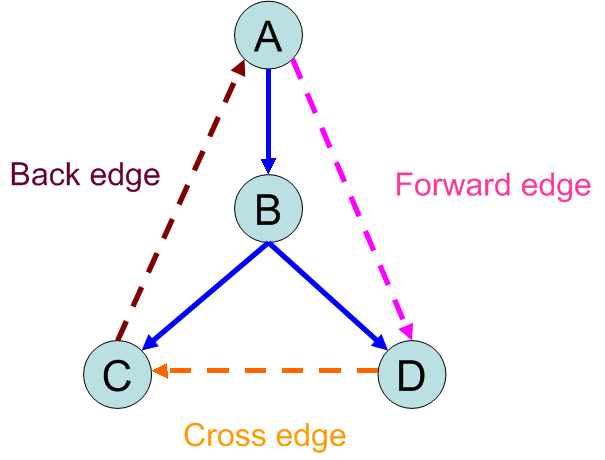
\includegraphics[scale=0.20]{figure/bfs_dfs/dfsdi} \\ \textcolor{red}{Back edge}}                              \\ \hline
    \end{tabular}
  \end{table}

\end{frame}


\begin{frame}
  \frametitle{Cycle detection problems}

  \begin{center}
    \textcolor{purple}{Using BFS on undirected graph for cycle detection:}
  \end{center}

  \begin{columns}
    \begin{column}{0.50\textwidth}
      \begin{figure}
        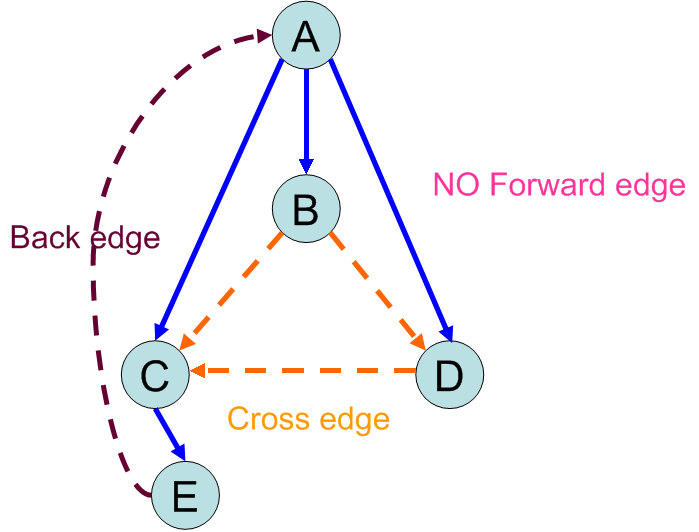
\includegraphics[scale=0.30]{figure/bfs_dfs/bfsdi}
        \caption{{\scriptsize BFS on digraph with back edges.}}
        \label{fig:bfsundirected}
      \end{figure}
    \end{column}

    \begin{column}{0.50\textwidth}
      \begin{figure}
        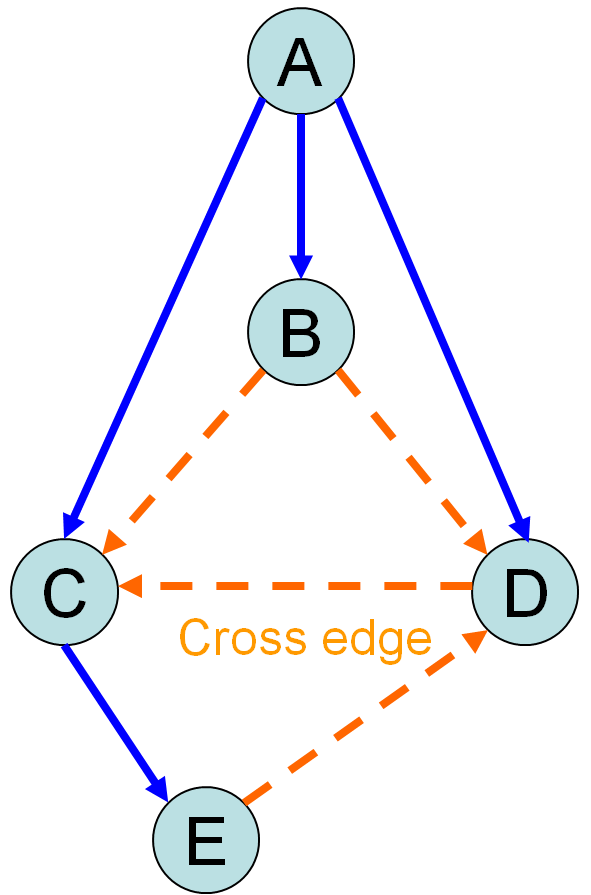
\includegraphics[scale=0.30]{figure/bfs_dfs/bfsdinoback}
        \caption{{\scriptsize BFS on digraph without back edges.}}
        \label{fig:bfsdinoback}
      \end{figure}
    \end{column}
  \end{columns}

\end{frame}




    %%%%%%%% Exploring types of edges on both BFS and DFS %%%%%%%
\subsection{Exploring DFS's Active Intervals}

\begin{frame}
  \frametitle{Exploring DFS's active intervals}

    \begin{figure}
      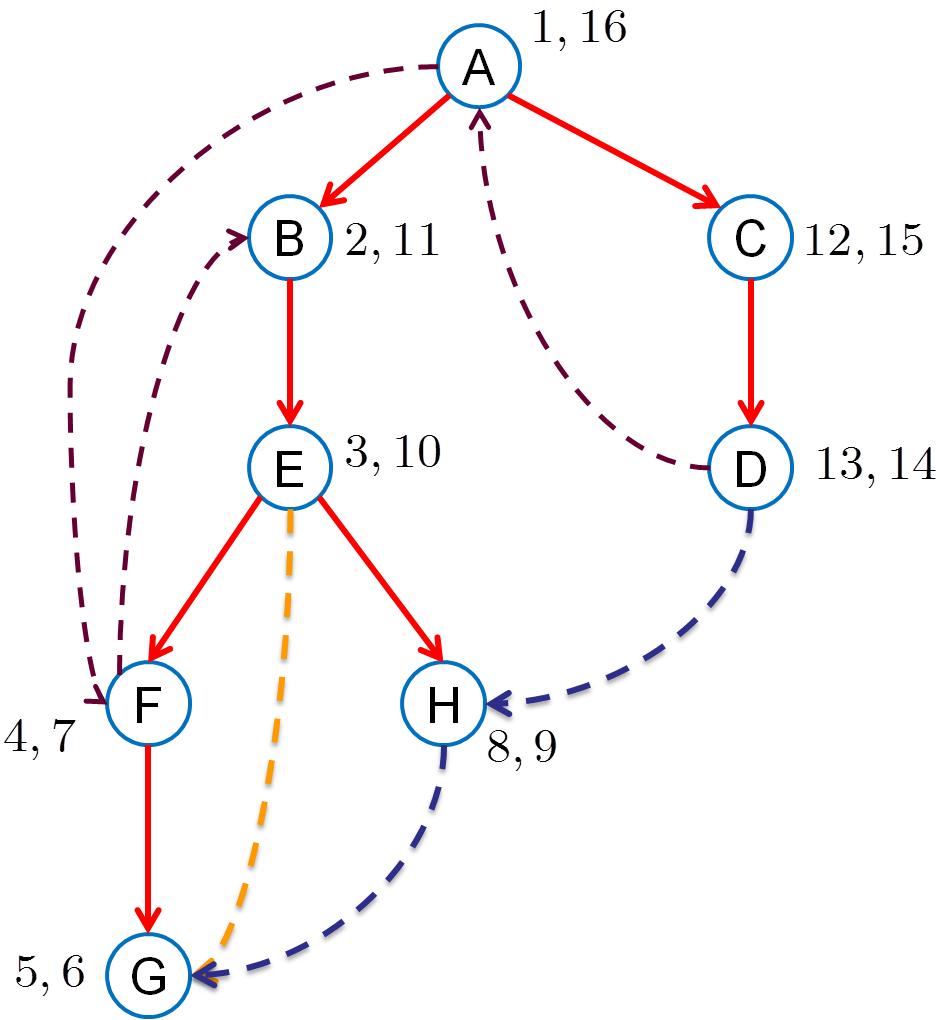
\includegraphics[scale=0.40]{figure/bfs_dfs/activeinterval}
      \caption{{\scriptsize Active intervals in DFS on digraph.}}
      \label{fig:activeinterval}
    \end{figure}

\end{frame}


\begin{frame}
  \frametitle{Exploring DFS's active intervals}

  \begin{enumerate}
    \item Who is ancestor ?
    \item How many descendants ?
      \pause
    \item topological sorting (on digraph)
    \item strongly-connected components (on digraph)
    \item biconnected components (on undirected graph)
  \end{enumerate}

\end{frame}


\subsubsection{DAG and Topological Sorting}
\begin{frame}
  \frametitle{DAG and topological sorting}

  \begin{enumerate}
    \setlength{\itemsep}{0.20cm}

    \item absence of back edges = acyclicity (DAG)
    \item topological sorting
      \begin{itemize}
        \item source, sink
      \end{itemize}
  \end{enumerate}

  \begin{figure}
    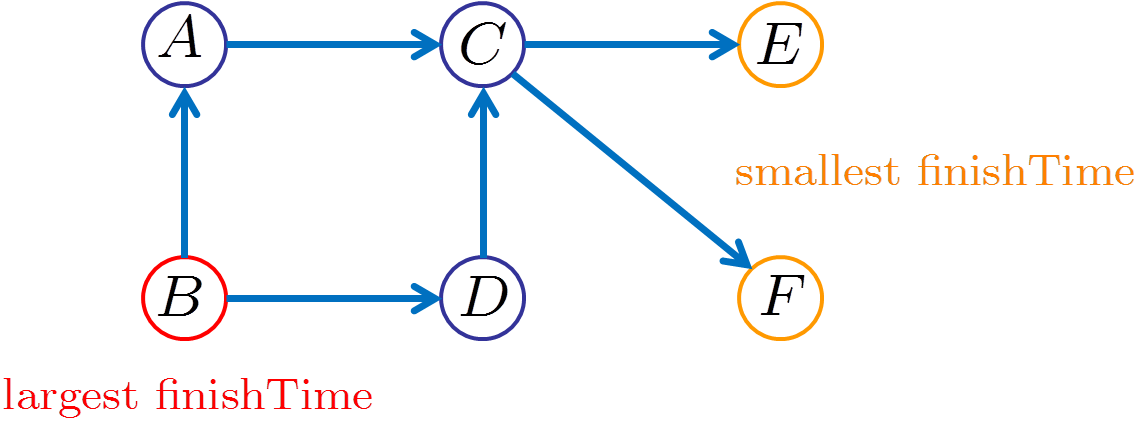
\includegraphics[scale=0.40]{figure/bfs_dfs/DAG}
    \caption{{\scriptsize Example of DAG.}}
    \label{fig:activeinterval}
  \end{figure}
      
\end{frame}

%    \item critical path
%      \begin{itemize}
%        \item longest path in DAG
%      \end{itemize}

%\begin{frame}
%  \frametitle{DAG and Topological Sorting}
%
%  \begin{columns}
%    \begin{column}{0.40\textwidth}
%      \begin{figure}
%        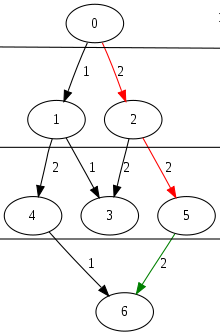
\includegraphics[scale=0.30]{figure/bfs_dfs/longestpath}
%        \caption{{\scriptsize DAG with distance layers.}}
%        \label{fig:longestpath}
%      \end{figure}
%    \end{column}
%
%    \begin{column}{0.60\textwidth}
%      \begin{figure}
%        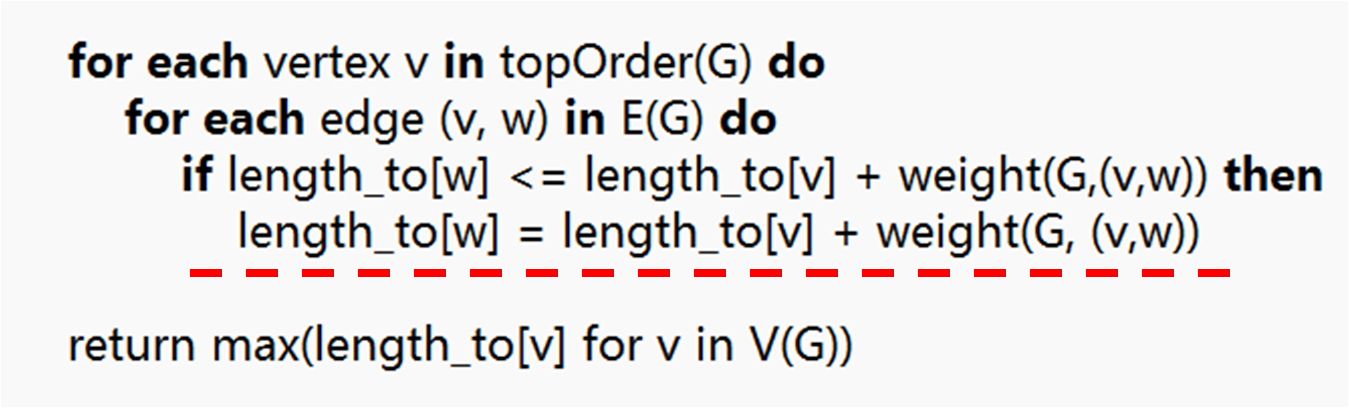
\includegraphics[scale=0.30]{figure/bfs_dfs/longestpathalg}
%        \caption{{\scriptsize Dag longest path algorithm.}}
%        \label{fig:longestpathalg}
%      \end{figure}
%    \end{column}
%
%  \end{columns}
%
%    \pause
%    \textcolor{purple}{In general graphs, longest path problem is NP-hard.}
%
%\end{frame}

\begin{frame}
  \frametitle{DAG and topological sorting}
  
  \begin{itemize}
    \item critical path $\to$ longest path in DAG
  \end{itemize}
  
  \pause
  \vspace{0.50cm}
  
  \textcolor{purple}{Note: In general graphs, longest path problem is NP-hard !}
    
\end{frame}

\subsubsection{Strongly Connected Components of a Digraph}

\begin{frame}
  \frametitle{SCC of digraph}

  \textcolor{purple}{``Two-trier'' structure of digraph} ([\textcolor{blue}{$P_{379}$ 7.22}]):

  \begin{figure}
    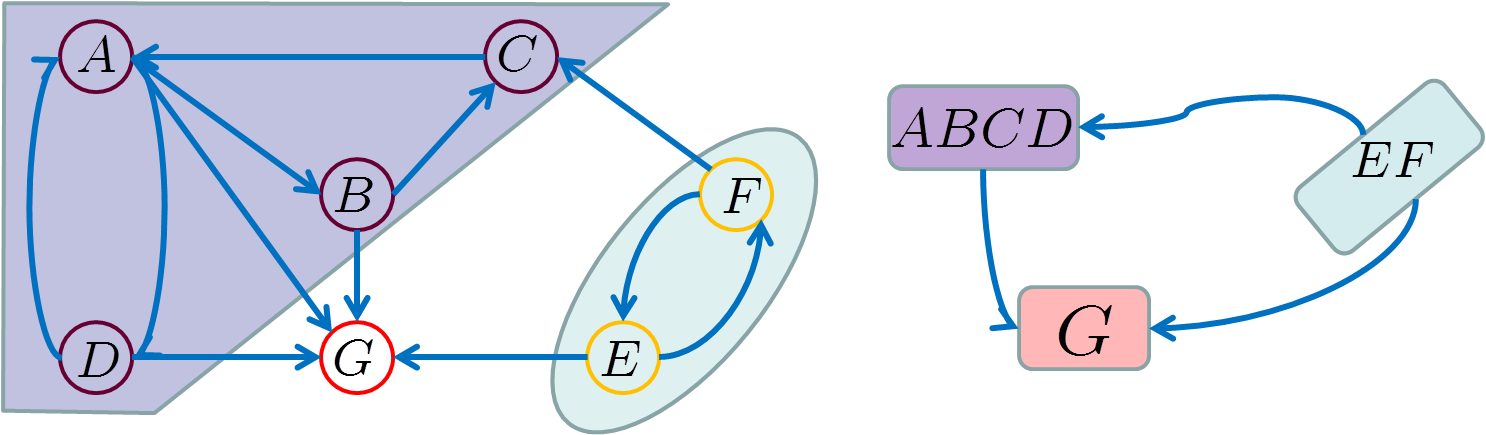
\includegraphics[scale=0.35]{figure/bfs_dfs/SCCDI}
    \label{fig:scc}
  \end{figure}

  \pause

{\small

  \begin{enumerate}
    \item ``The node that has \textcolor{red}{highest} finishTime in DFS must lie in a \textcolor{red}{source SCC''};
    \pause
    \item What we need is sink! So try \textcolor{red}{$G^R$}; ([\textcolor{blue}{$P_{380}$ 7.26}])
    \item When a sink SCC is found (by connectivity), just delete it and continue \textcolor{red}{recursively}.
  \end{enumerate}
}

\end{frame}


\subsubsection{Biconnected Components of an Undirected Graph}

\begin{frame}
  \frametitle{Biconnected components of an undirected graph}

  \textcolor{purple}{Algorithms for biconnected components:}
  \begin{description}
    \setlength{\itemsep}{0.20cm}
    \item [Brute force:] try every vertex and check connectivity: $O \big( n(m+n) \big )$.
    \item [Clever approach:] single DFS making use of \textcolor{blue}{\emph{back edges and active intervals}}.
  \end{description}

\end{frame}


\begin{frame}
  \frametitle{Biconnected components of an undirected graph}

    \begin{columns}
      \begin{column}{0.50\textwidth}
         \begin{figure}
            \begin{center}
              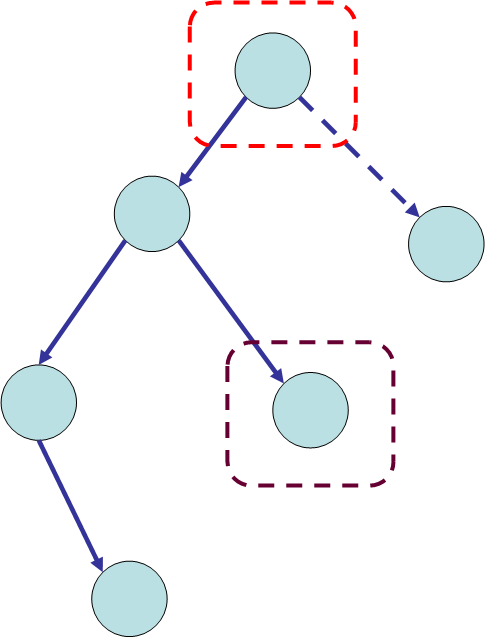
\includegraphics[scale=0.30]{figure/bfs_dfs/dfsbiconn}
              \caption{What if DFS tree is the entirety of the graph ?}
              \label{fig:dfsbiconn}
            \end{center}
          \end{figure}
      \end{column}

      \begin{column}{0.50\textwidth}
          \begin{figure}
            \begin{center}
              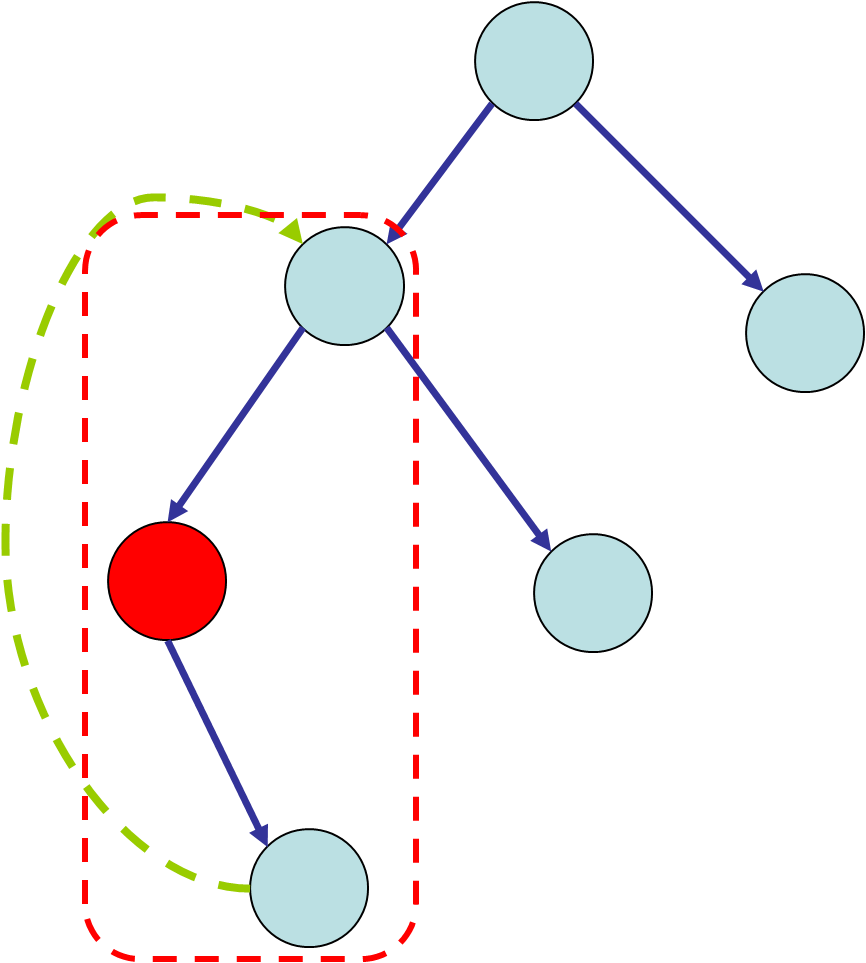
\includegraphics[scale=0.30]{figure/bfs_dfs/backedgebiconn}
              \caption{Back edge, cycle, no articulation vertices.}
              \label{fig:backedgebiconn}
            \end{center}
          \end{figure}
      \end{column}

    \end{columns}

\end{frame}


%\begin{frame}
%  \frametitle{Biconnected components of an undirected graph}
%
%  \textcolor{purple}{Important information:}
%
%  \textcolor{blue}{the extend to which back edges link chunks of the DFS tree back to ancestor nodes:}
%  \begin{enumerate}
%    \setlength{\itemsep}{0.20cm}
%
%    \item $v$ is first discovered.
%        \[
%          back = discoverTime(v).
%        \]
%    \item back edge $vw$.
%        \[
%          back = min(back, discoverTime(w)).
%        \]
%    \item backtracking from $w$ to $v$.
%        \[
%          back = min(back, wback).
%        \]
%  \end{enumerate}
%
%\end{frame}


\begin{frame}
  \frametitle{Biconnected components of an undirected graph}
  
  \begin{figure}
    \begin{center}
      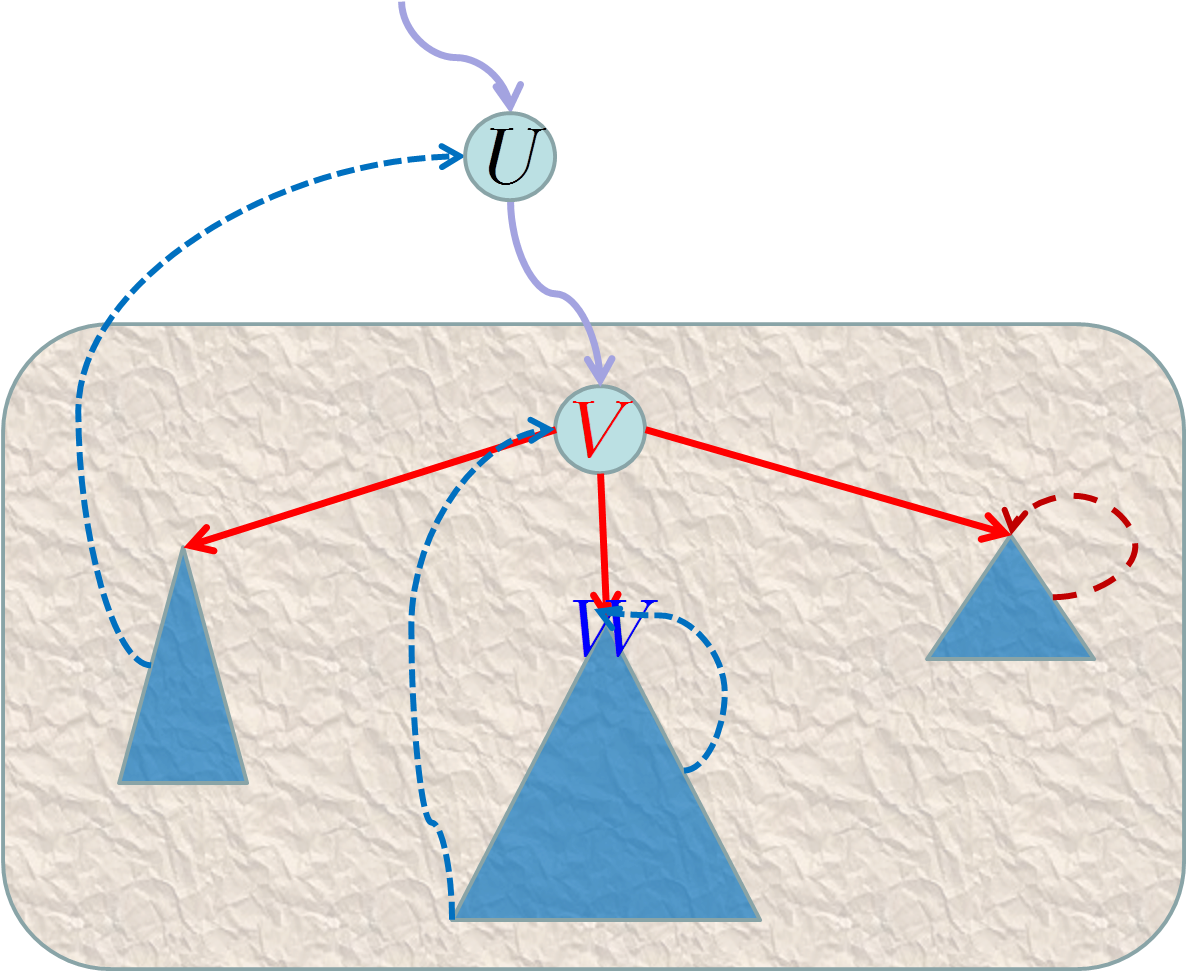
\includegraphics[scale=0.40]{figure/bfs_dfs/bicon1}
      \caption{{\scriptsize Three cases of articulations (1).}}
      \label{fig:bicon1}
    \end{center}
  \end{figure}  
  
\end{frame}


\begin{frame}
  \frametitle{Biconnected components of an undirected graph}

  \begin{figure}
    \begin{center}
      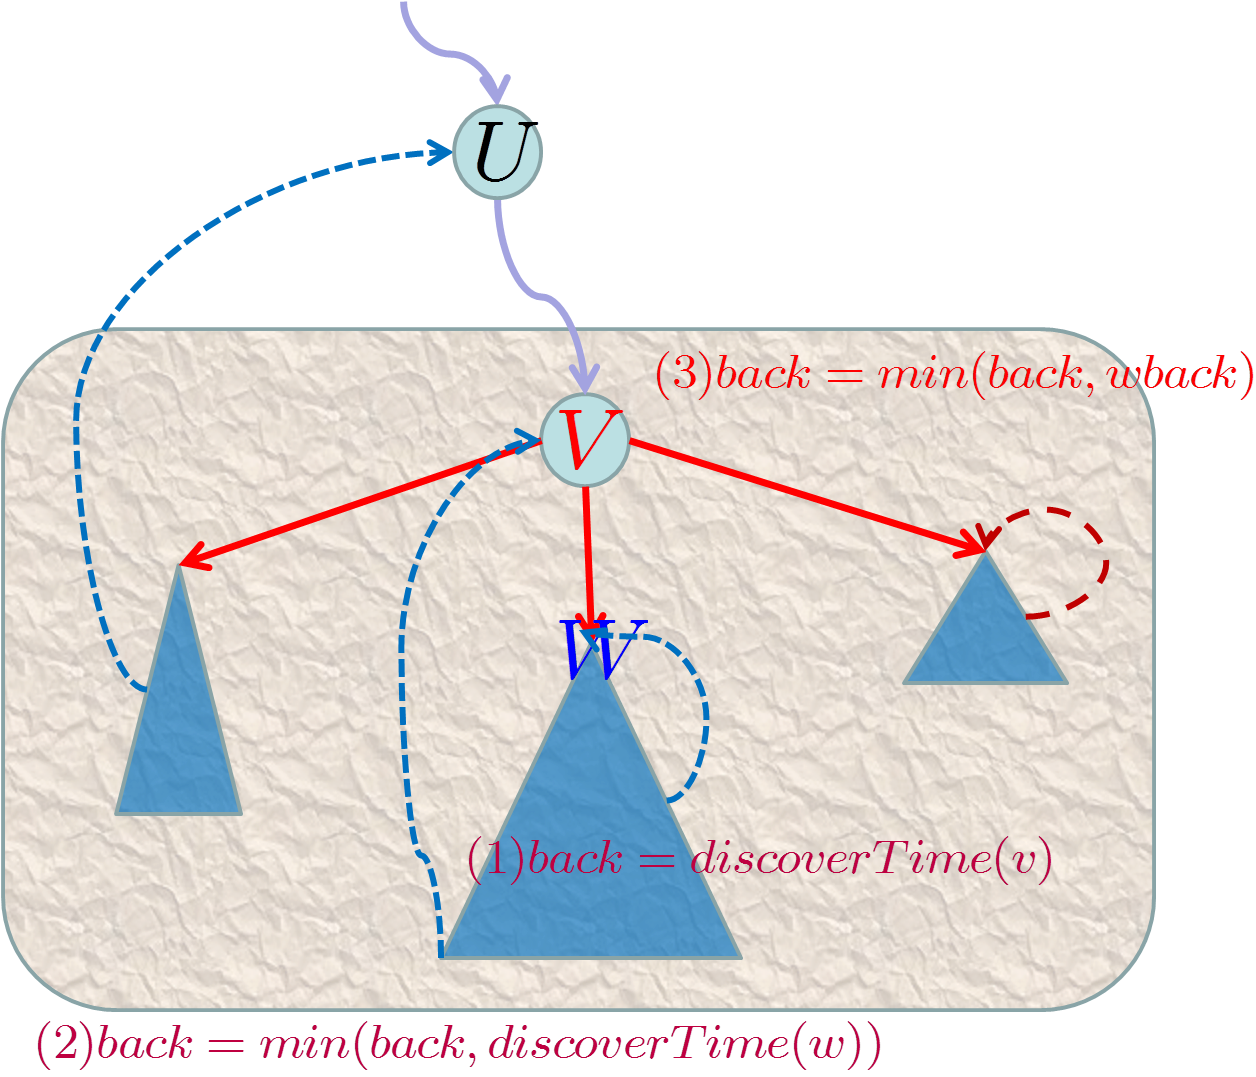
\includegraphics[scale=0.40]{figure/bfs_dfs/bicon2}
      \caption{{\scriptsize Three cases of articulations (2).}}
      \label{fig:bicon2}
    \end{center}
  \end{figure}

\end{frame}


\begin{frame}
  \frametitle{Biconnected components of an undirected graph}

  \begin{figure}
    \begin{center}
      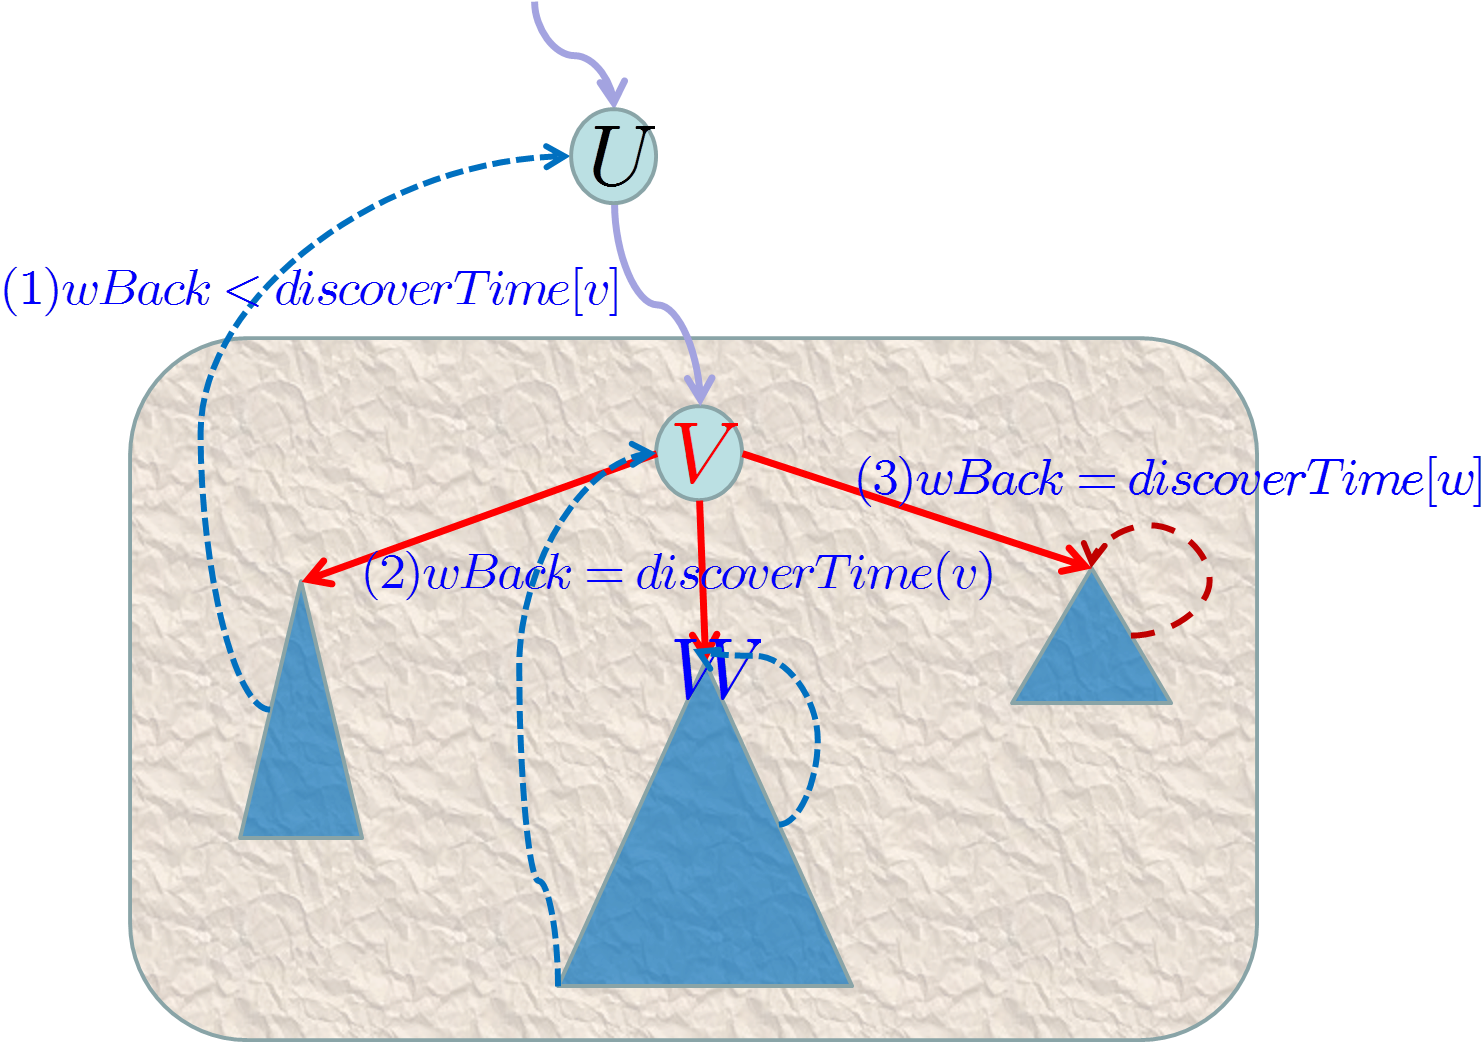
\includegraphics[scale=0.40]{figure/bfs_dfs/bicon3}
      \caption{{\scriptsize Three cases of articulations (3).}}
      \label{fig:bicon3}
    \end{center}
  \end{figure}

\end{frame}



\begin{frame}
  \frametitle{Biconnected components of an undirected graph}

  \begin{figure}
    \begin{center}
      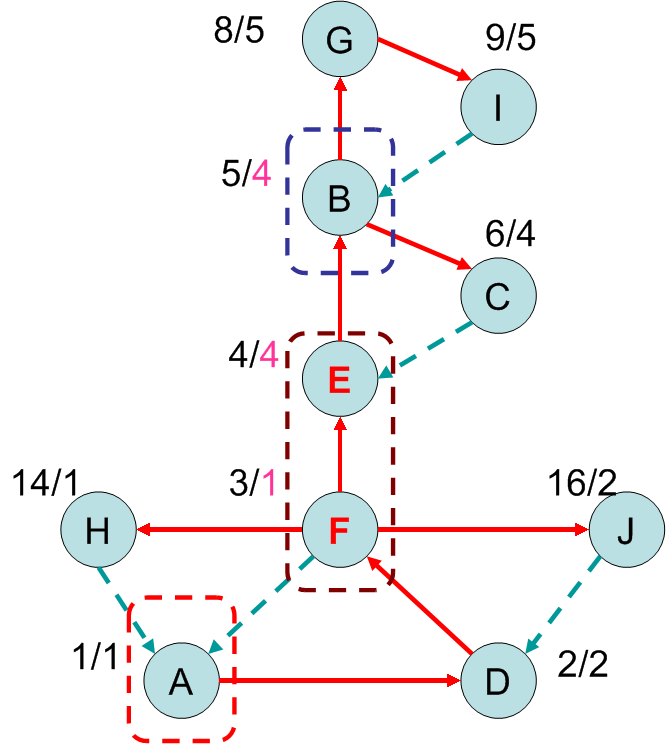
\includegraphics[scale=0.30]{figure/bfs_dfs/articulationex}
      \caption{Three cases of articulations.}
      \label{fig:articulations}
    \end{center}
  \end{figure}

\end{frame}


\begin{frame}
  \frametitle{Biconnected components of an undirected graph}

  \textcolor{purple}{Q:} How the reachability relation impacts whether $v$ is an articulation vertex ?
  \begin{enumerate}
    \item Root cut-nodes ([\textcolor{blue}{$P_{382}$ 7.37}]).
    \item Bridge cut-nodes.
    \item Parent cut-nodes.
  \end{enumerate}

  \pause
  \vspace{0.40cm}

    Q : $\textrm{Back } \ge \textrm{discoverTime} \lbrack v \rbrack$ ([\textcolor{blue}{$P_{383}$ 7.42}]).

  \pause

    A : $\textrm{Back } = \textrm{discoverTime} \lbrack v \rbrack$. It just detects Bridge cut-nodes.

\end{frame} 
%%%%%%%%%%%%%%%%%%%%%%%%%%%%%%%%%%%%%%%%%%%%%%%%%%%%%%%%%%%%%%%%%%%%%
%%%%%%%%%%%%%%%%%%%%%%% Minimum Spanning Tree %%%%%%%%%%%%%%%%%%%%%%%

\section{Minimum Spanning Tree}

\begin{frame}
  \frametitle{Minimum Spanning Tree}

    \begin{itemize}

    \item (\textcolor{purple}{Evaluate Prim's MST algorithm implemented with min-heap} ([\textcolor{blue}{$P_{417}$ 8.9}]):) \\
        \begin{enumerate}
          \item Find the asymptotic order of the number of comparisons of edge weights in the worst case.
          \item Find the asymptotic order of the number of comparisons of edge weights on a \textcolor{blue}{bounded-degree} family.
          \item Find the asymptotic order of the number of comparisons of edge weights on a \textcolor{blue}{planar graph}.
        \end{enumerate}

    \end{itemize}

\end{frame}



\begin{frame}
  \frametitle{Minimum Spanning Tree}

    \[
      T(n,m) = O \big (nT(getMin) + nT(deleteMin) + mT(decreaseKey) \big ). (\lbrack \textcolor{blue}{P_{395}} \rbrack)
    \]

    \pause

    \begin{itemize}
      \item $getMin: O(1)$.  \\  \emph{no comparison of edge weights}.
      \item $deleteMin: O(\log n)$.  \\  \textcolor{red}{NOT}: $O(\log m)$.
      \item $decreaseKey: O(\log n)$.  \\ \textcolor{red}{NOT}: $O(n + \log n)$ where $O(n)$ for search ([\textcolor{blue}{$P_{296}$}]).
      \item ``Else if newWgt less than fringeWgt for w'' ([\textcolor{blue}{$P_{395}$}]) : $O(m).$
      \item \textcolor{blue}{In total,}
      \[
      T(n,m) = O(n \log n + m \log n + 2m) = O((n+m) \log n).
      \]
    \end{itemize}

\end{frame}



\begin{frame}
  \frametitle{Minimum Spanning Tree}

  \begin{itemize}
      \item
        $m \le \frac{nk} {2}, \Rightarrow T(n,m) = O((n+m) \log n) = O((n+ \frac{nk}{2}) \log n) = O(n \log n).$

        \pause

      \item
        First, we should know the relation between $m$ and $n$.
        \begin{equation}
          n - m + f = 2. \label{eq: EulerExtension}
        \end{equation}

        If $deg(f_i) \ge l$,
        \begin{equation}
          2m = \sum_{i=1}^f deg(R_i) \ge lf. \label{eq: Handshaking}
        \end{equation}
        \begin{equation}
          m \le \frac{l}{l-2}(n-2)
        \end{equation}

        \pause

        If $G$ is tree, $m=n-1$; Else, $l \ge 3$.
        \begin{equation}
          \textcolor{blue}{m \le \frac{l}{l-2}(n-2) \le 3(n-2) = 3n - 6}
        \end{equation}
        \[
          T(n,m) = O((n+m) \log n) = O((n + 3n) \log n) = O(n \log n).
        \]
  \end{itemize}

\end{frame} 
%%%%%%%%%%%%%%%%%%%%%%%%%%%%%%%%%%%%%%%%%%%%%%%%%%%%%%%%%%%%%%%%%%%%%
%%%%%%%%%%%%%%%%%%%%%%%%% Shortest Paths %%%%%%%%%%%%%%%%%%%%%%%%%%

\section{Shortest Paths}

\begin{frame}
  \frametitle{Shortest paths}

  \textcolor{purple}{Different editions of shortest paths problems:}
  \begin{enumerate}
    \item shortest(longest) path in DAG  \\
      \emph{\textcolor{blue}{Dynamic Programming}}
    \item single-source shortest paths
      \begin{itemize}
        \item No negative edges. \\
          \emph{\textcolor{blue}{Dijkstra algorithm.}}
        \item With negative edges (No negative cycle). \\
          \emph{\textcolor{gray}{Bellman-Ford algorithm.}}
      \end{itemize}
    \item all pairs shortest paths \\
      \emph{\textcolor{blue}{Floyd-Warshall algorithm.}}
  \end{enumerate}

\end{frame}

%\begin{frame}
%  \frametitle{Shortest paths}
%
%  \textcolor{purple}{To better understand these problems and algorithms:}
%  \vspace{0.40cm}
%
%  \begin{enumerate}
%    \setlength{\itemsep}{0.30cm}
%    \item Why the algorithm works for this problem ?
%    \item Does the algorithm also work for another problem ?
%  \end{enumerate}
%
%\end{frame}


\begin{frame}
  \frametitle{Shortest paths}

  \textcolor{purple}{DAG can be topologically sorted, so \emph{DP} works.}

  \begin{figure}
    \begin{center}
      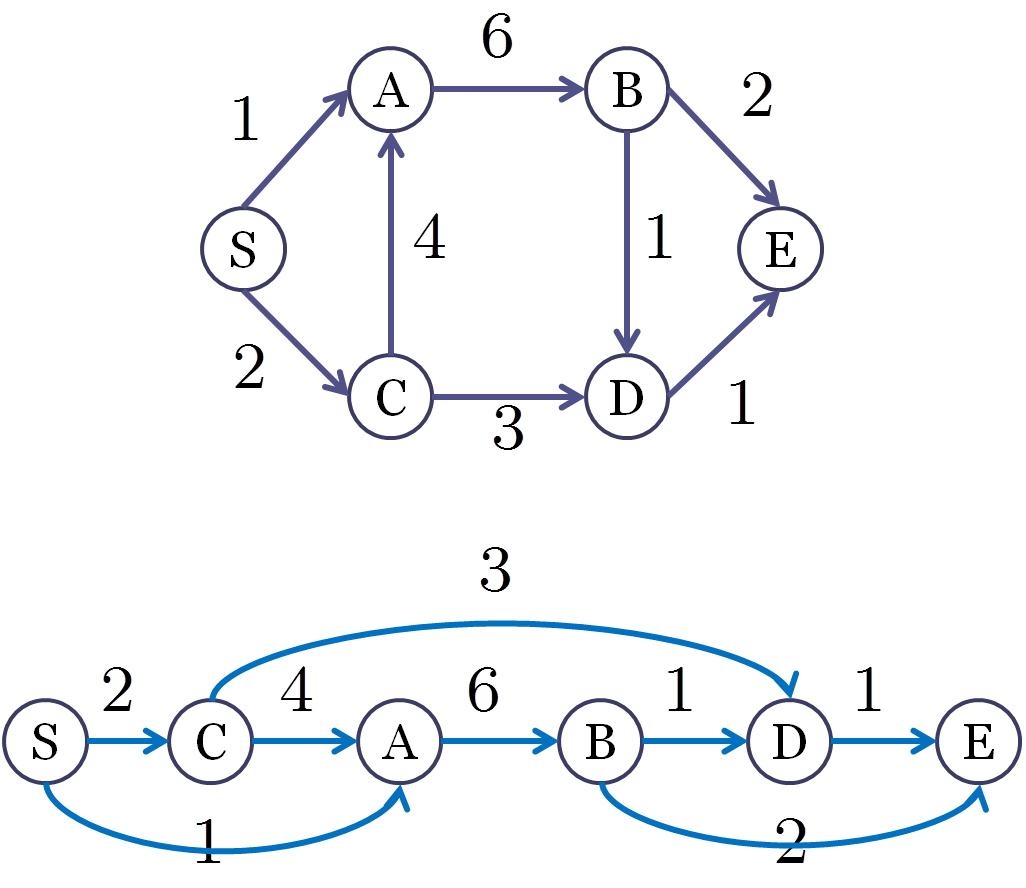
\includegraphics[scale=0.30]{figure/bfs_dfs/daglinear}
      \caption{{\scriptsize A dag and its topological sorting.}}
      \label{fig:daglinear}
    \end{center}
  \end{figure}

  \[
    dist(D) = \min \lbrace dist(B)+1, dist(C)+3 \rbrace.
  \]

\end{frame}


\begin{frame}
  \frametitle{Shortest paths}

  \textcolor{purple}{Shortest path without negative edges : \emph{Dijkstra algorithm}}

  \begin{figure}
    \begin{center}
      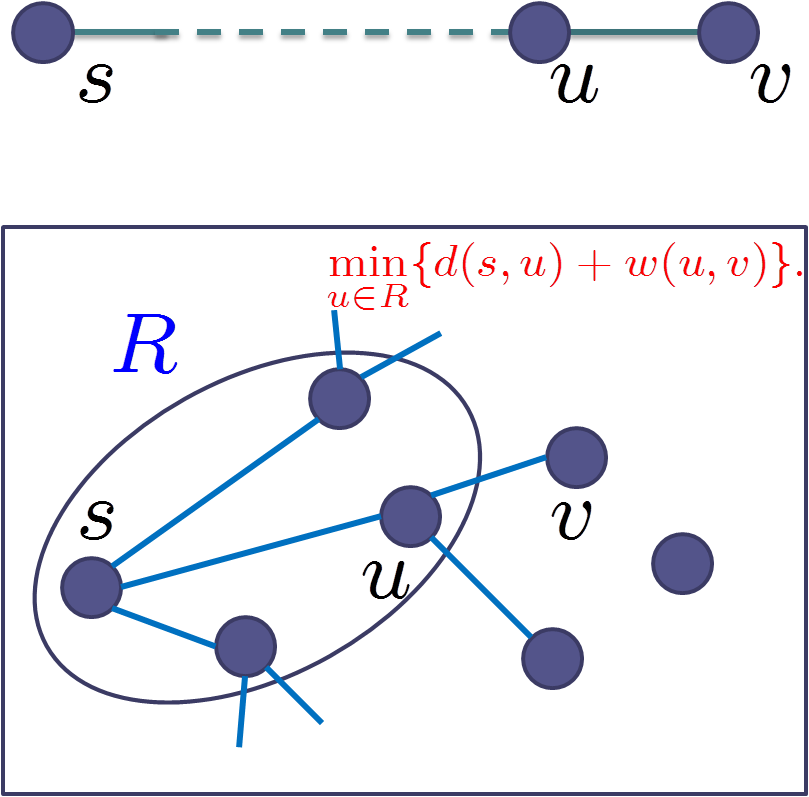
\includegraphics[scale=0.40]{figure/bfs_dfs/dijkstra}
      \caption{{\scriptsize Property of shortest paths.}}
      \label{fig:dijkstra}
    \end{center}
  \end{figure}

\end{frame}


\begin{frame}
  \frametitle{Priority queue implementations}

  \textcolor{purple}{Complexity of Dijkstra algorithm:}
  \begin{enumerate}
    \item makequeue, $\lvert V \rvert \cdot insert$
    \item $\lvert V \rvert \cdot deletemin$
    \item $\lvert E \rvert \cdot descreaseKey$
  \end{enumerate}

  \pause
  \vspace{0.50cm}

  \textcolor{purple}{Different implementations of priority queue:}

  {\scriptsize

    \begin{tabular}{|c||c|c|c|}
      \hline
      Implementation     & deletemin        & insert, decreaseKey       & total                 \\ \hline \hline
      Array              & $O(V)$           & $O(1)$                    & $O(V^2)$              \\ \hline
      Binary heap        & $O(\log{V})$     & $O(\log{V})$              & $O((V+E) \log {V})$   \\ \hline
      Fibonacci heap     & $O(\log{V})$     & $O(1)$                    & O$(V \log {V} + E)$   \\
      \hline
    \end{tabular}
  }

\end{frame}


\begin{frame}
  \frametitle{Shortest path with negative edges: \emph{Bellman-Ford algorithm}}

  \begin{figure}
    \begin{center}
      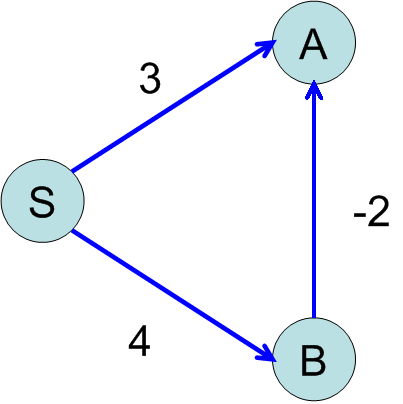
\includegraphics[scale=0.40]{figure/bfs_dfs/dijkstranegative}
      \caption{{\scriptsize Dijkstra algorithm fails if there are negative edges ([\textcolor{blue}{$P_{418}$ 8.14}]).}}
      \label{fig:dijkstranegative}
    \end{center}
  \end{figure}

\end{frame}



\begin{frame}
  \frametitle{All pairs of shortest paths: \emph{Floyd-Warshall algorithm}}

  \begin{figure}
    \begin{center}
      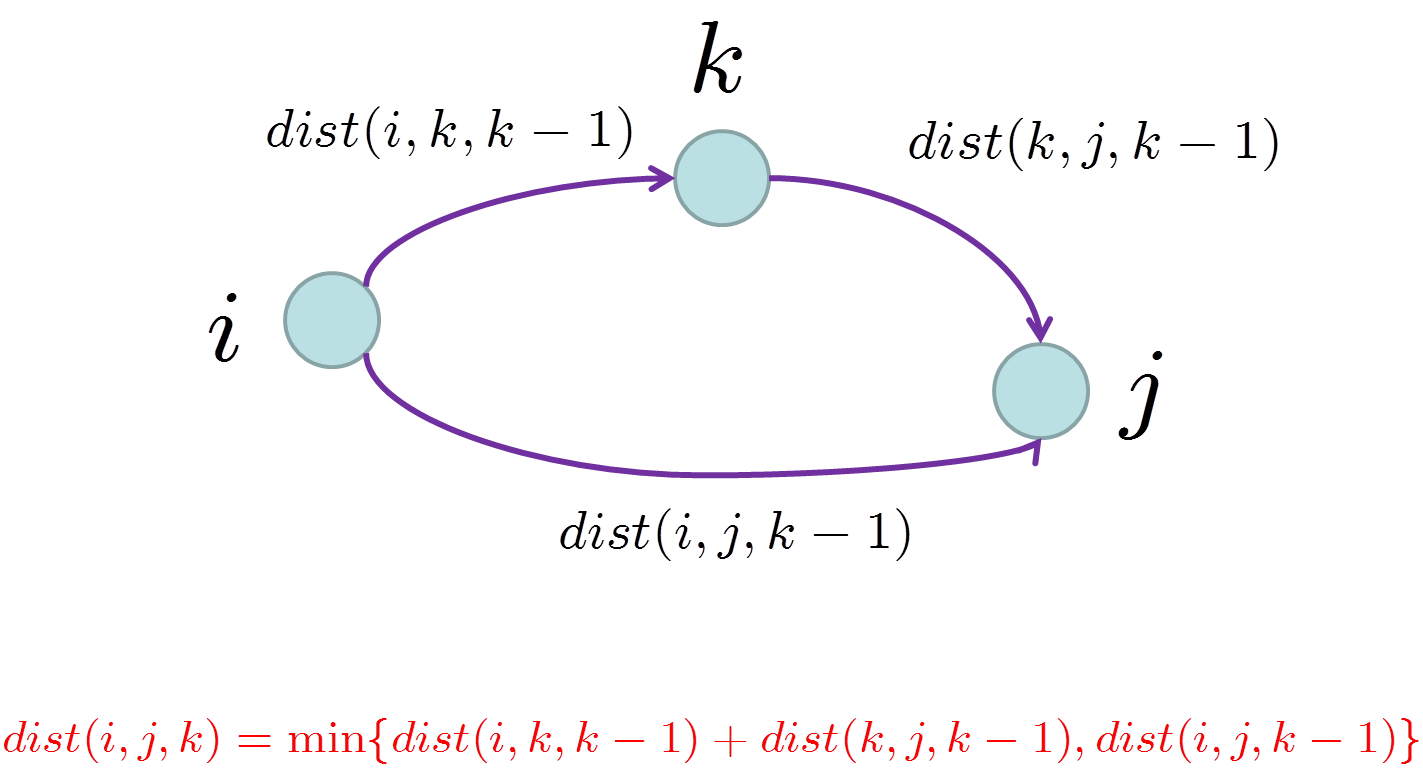
\includegraphics[scale=0.40]{figure/bfs_dfs/warshall}
      \label{fig:warshall}
    \end{center}
  \end{figure}

  \pause
  \vspace{0.40cm}
  \textcolor{red}{Assumption: No negative cycles.}

\end{frame}


\begin{frame}
  \frametitle{All pairs of shortest paths: \emph{Floyd-Warshall algorithm}}

  \begin{itemize}
    \item Routing table for all-pair shortest path ([\textcolor{blue}{$P_{448}$ 9.10}]).
    \item Length of shortest cycle in digraph ([\textcolor{blue}{$P_{448}$ 9.12}]).
  \end{itemize}

\end{frame}



\begin{frame}
  \frametitle{All pairs of shortest paths: \emph{Floyd-Warshall algorithm}}

  \begin{itemize}
    \item Routing table for all-pair shortest path ([\textcolor{blue}{$P_{448}$ 9.10}]).
    \vspace{0.50cm}

      \begin{figure}
        \begin{center}
          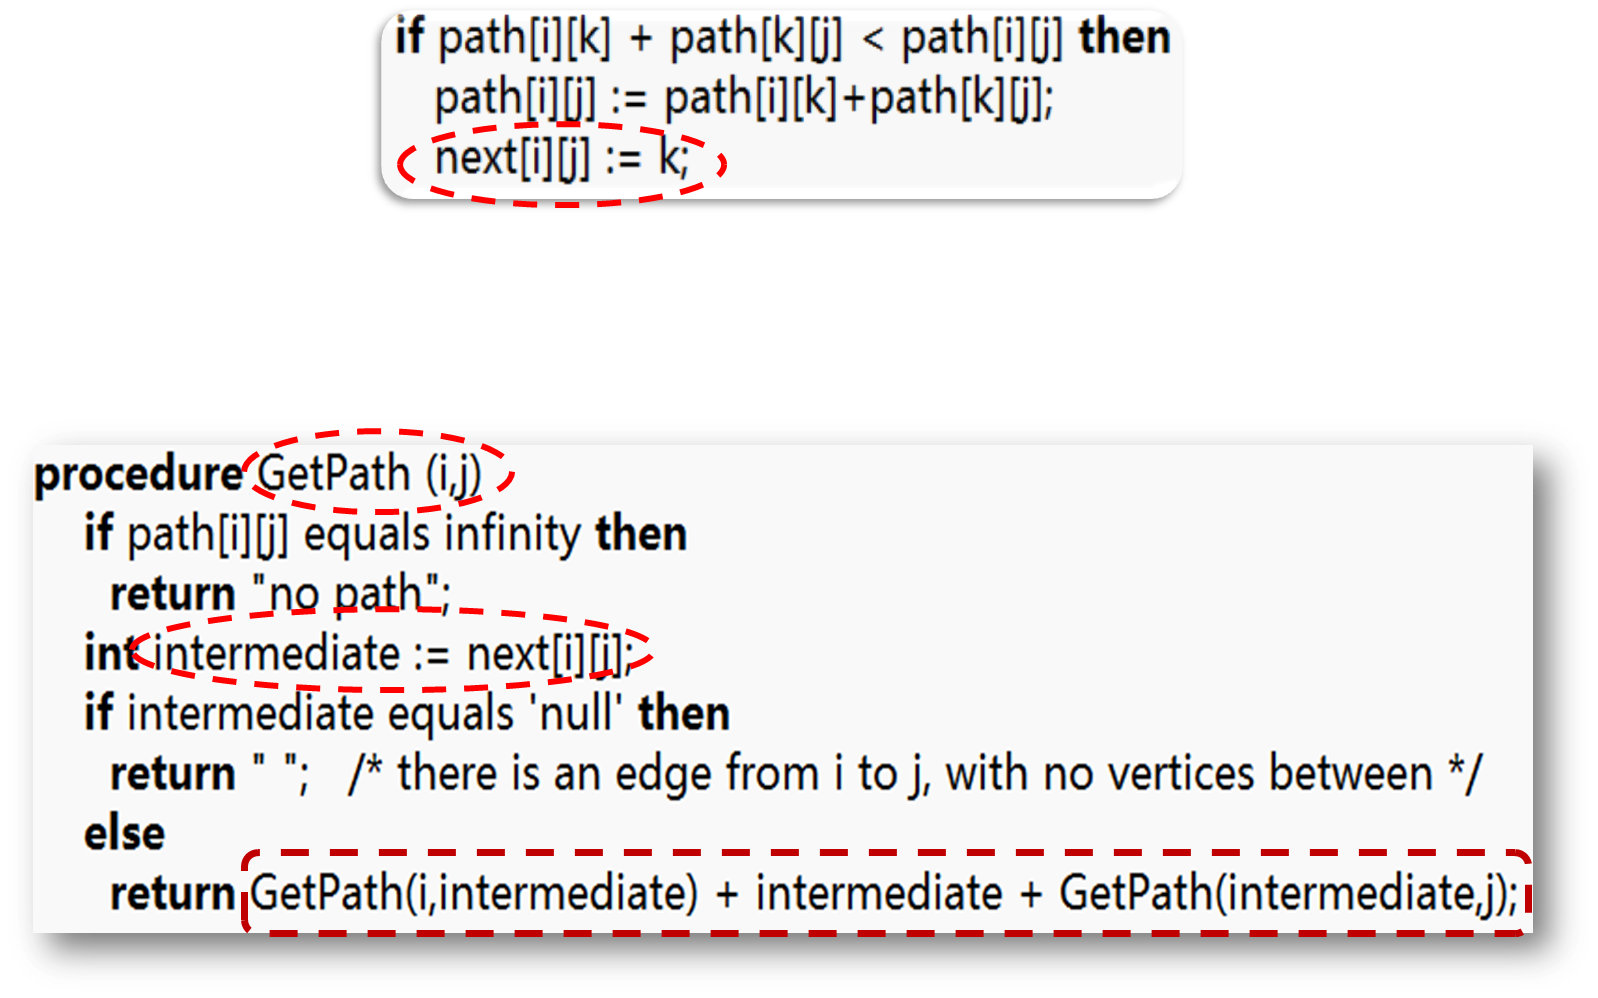
\includegraphics[scale=0.35]{figure/shortest_paths/route0}
          \caption{{\scriptsize Construction of routing table.}}
          \label{fig:route0}
        \end{center}
      \end{figure}
    \end{itemize}

\end{frame}



\begin{frame}
  \frametitle{All pairs of shortest paths: \emph{Floyd-Warshall algorithm}}

  \begin{itemize}
    \item Length of shortest cycle in digraph ([\textcolor{blue}{$P_{448}$ 9.12}]).
    \[
      path \lbrack i \rbrack \lbrack i \rbrack
    \]
    \[
      path \lbrack i \rbrack \lbrack i \rbrack < 0 ?
    \]
    \textcolor{red}{Fail for undirected graph:}
    \[
      \lbrace v, w \rbrace \to (v,w,v).
    \]
  \end{itemize}

\end{frame}


\begin{frame}
  \begin{figure}
    \begin{center}
      
\includegraphics[scale=0.60]{figure/thank}
      \label{fig:thank}
    \end{center}
  \end{figure}
\end{frame} 
%%%%%%%%%%%%%%%%%%%%%%%%%%%%%%%%%%%%%%%%%%%%%%%%%%%%%%%%%%%%%%%%%%%%%
% \include{}
%%%%%%%%%%%%%%%%%%%%%%%%%%%%%%%%%%%%%%%%%%%%%%%%%%%%%%%%%%%%%%%%%%%%%



%%%%%%%%%%%%%%%%%%%%%%%%%%%%%%%%%%%%%%%%%%%%%%%%%%%%%%%%%%%%%%%%%%%%%

%%%%%%%%%%%%%%%%%%%%%%%%%%%%%%%%%%%%%%%%%%%%%%%%%%%%%%%%%%%%%%%%%%%%%
\bibliographystyle{alpha}
\bibliography{bib4graphalg}
%%%%%%%%%%%%%%%%%%%%%%%%%%%%%%%%%%%%%%%%%%%%%%%%%%%%%%%%%%%%%%%%%%%%%

\end{document}
